\section{Microcomputer Organization } 
\subsection{Base Microcomputer Structure \embsys{81}{3.1}}
\begin{minipage}{0.7\linewidth}
	\begin{itemize}
		\item Central Processing Unit (\acs{CPU})
		\subitem Fetches, Decodes and Executes instructions from memory
		\item System Memory
		\subitem Program memory
		\subitem Data memory 
		\item Input-Output Subsystem
		\subitem Connect to the external world
		\item System Buses 
		\subitem Address bus (Indicate Adresse to be accessed)
		\subitem Data bus (carry Data or Instruction)
		\subitem Control bus (regualte activity on buses)
		\item Power \& Support Logic
	\end{itemize}
\end{minipage}
\begin{minipage}{0.3\linewidth}
	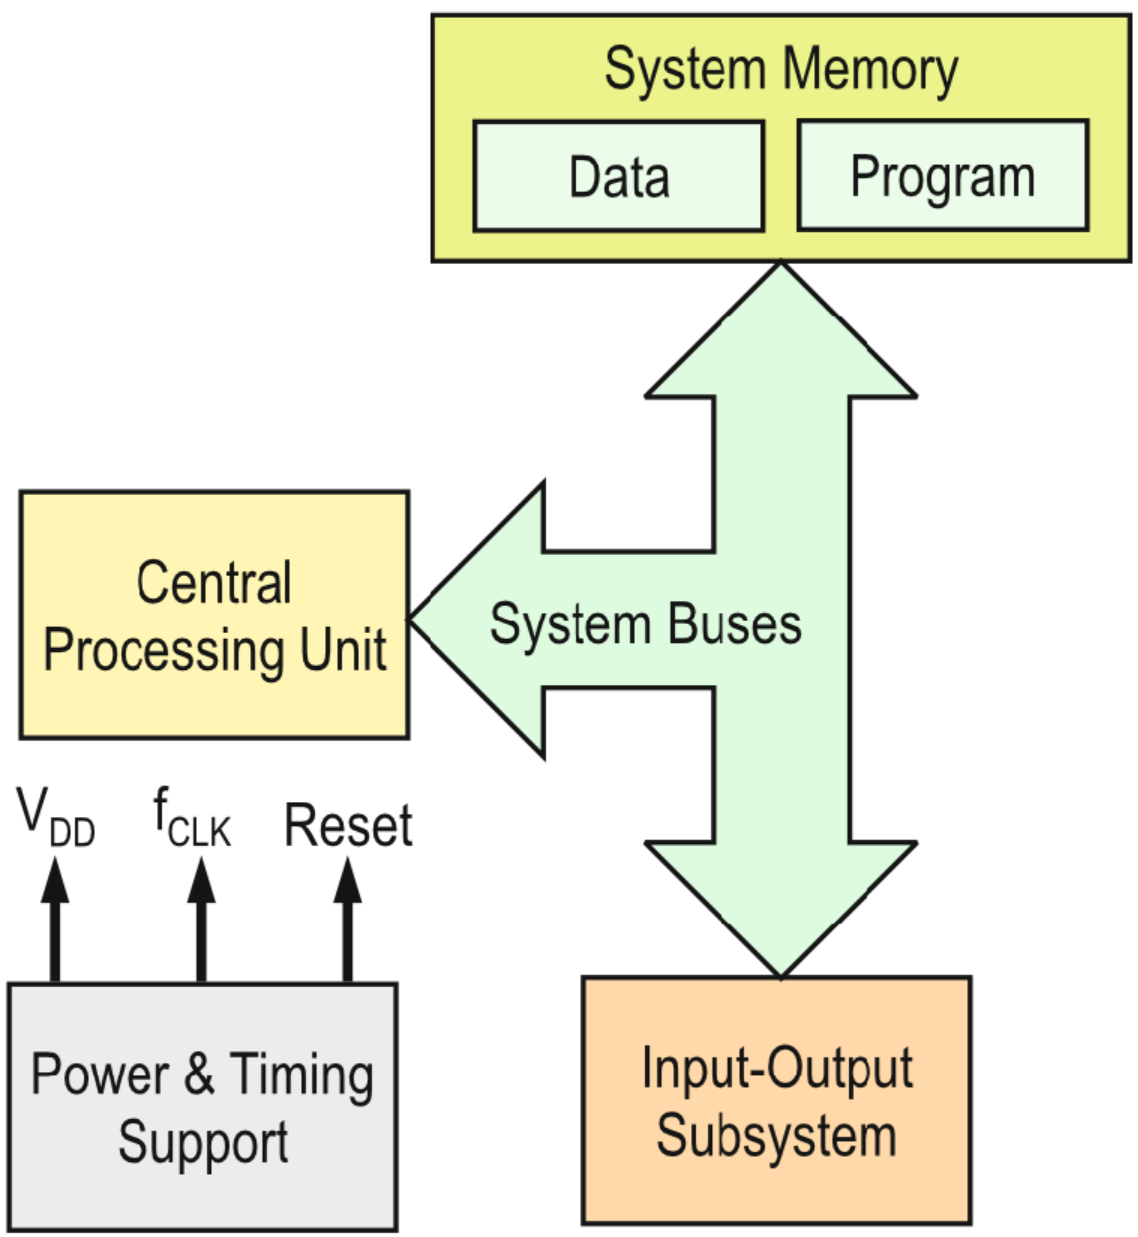
\includegraphics[width=\linewidth]{images/uCArchitecture} 
\end{minipage}
\subsection{Microcontroller vs. Microprocessors \embsys{82}{3.2}}
\begin{multicols}{2}
		\subsubsection{Microprocessor (\acs{MPU}, $\mu$P) }
		\begin{itemize}
			\item Contain a General Purpose \acs{CPU}
			\subitem \acs{ALU}, \acs{CU}, Registers, Bus Interface Logic
			\item Require External Components to form a Basic System
			\subitem Buses
			\subitem Memory
			\subitem \acs{I/O} Interface \& Devices
			\item Additional Characteristics
			\subitem Architecture optimized for \newline accelerating data processing
			\subitem Include elements to accelerate instruction execution  
		\end{itemize}
\subsubsection{Microcontroller (\acs{MCU},  $\mu$C)}
		\begin{itemize}
			\item Contain a Microprocessor Core
			\subitem Usually less complex than that of an \acs{MPU}
			\item Include memory and peripherals in a single chip
			\subitem Denominated $ computer-on-a-chip $ 
			\subitem Most \acs{MCU}s do not provide external buses
			\item On-chip Memory
			\subitem Includes both, Program and Data-memory
			\item Typical Peripherals
			\subitem Timers
			\subitem \acs{I/O} ports
			\subitem Data converters
		\end{itemize}
\end{multicols}

    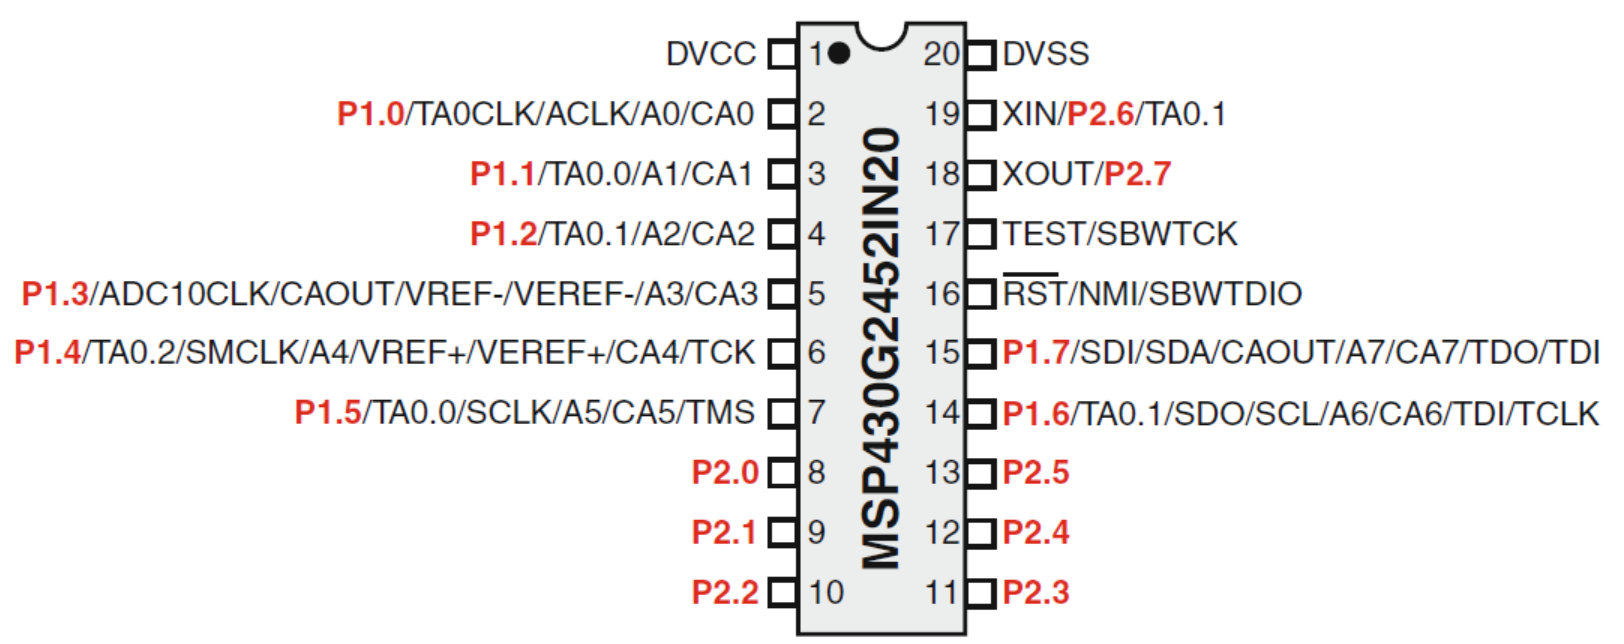
\includegraphics[width=10.5cm]{images/msp430hardware}
	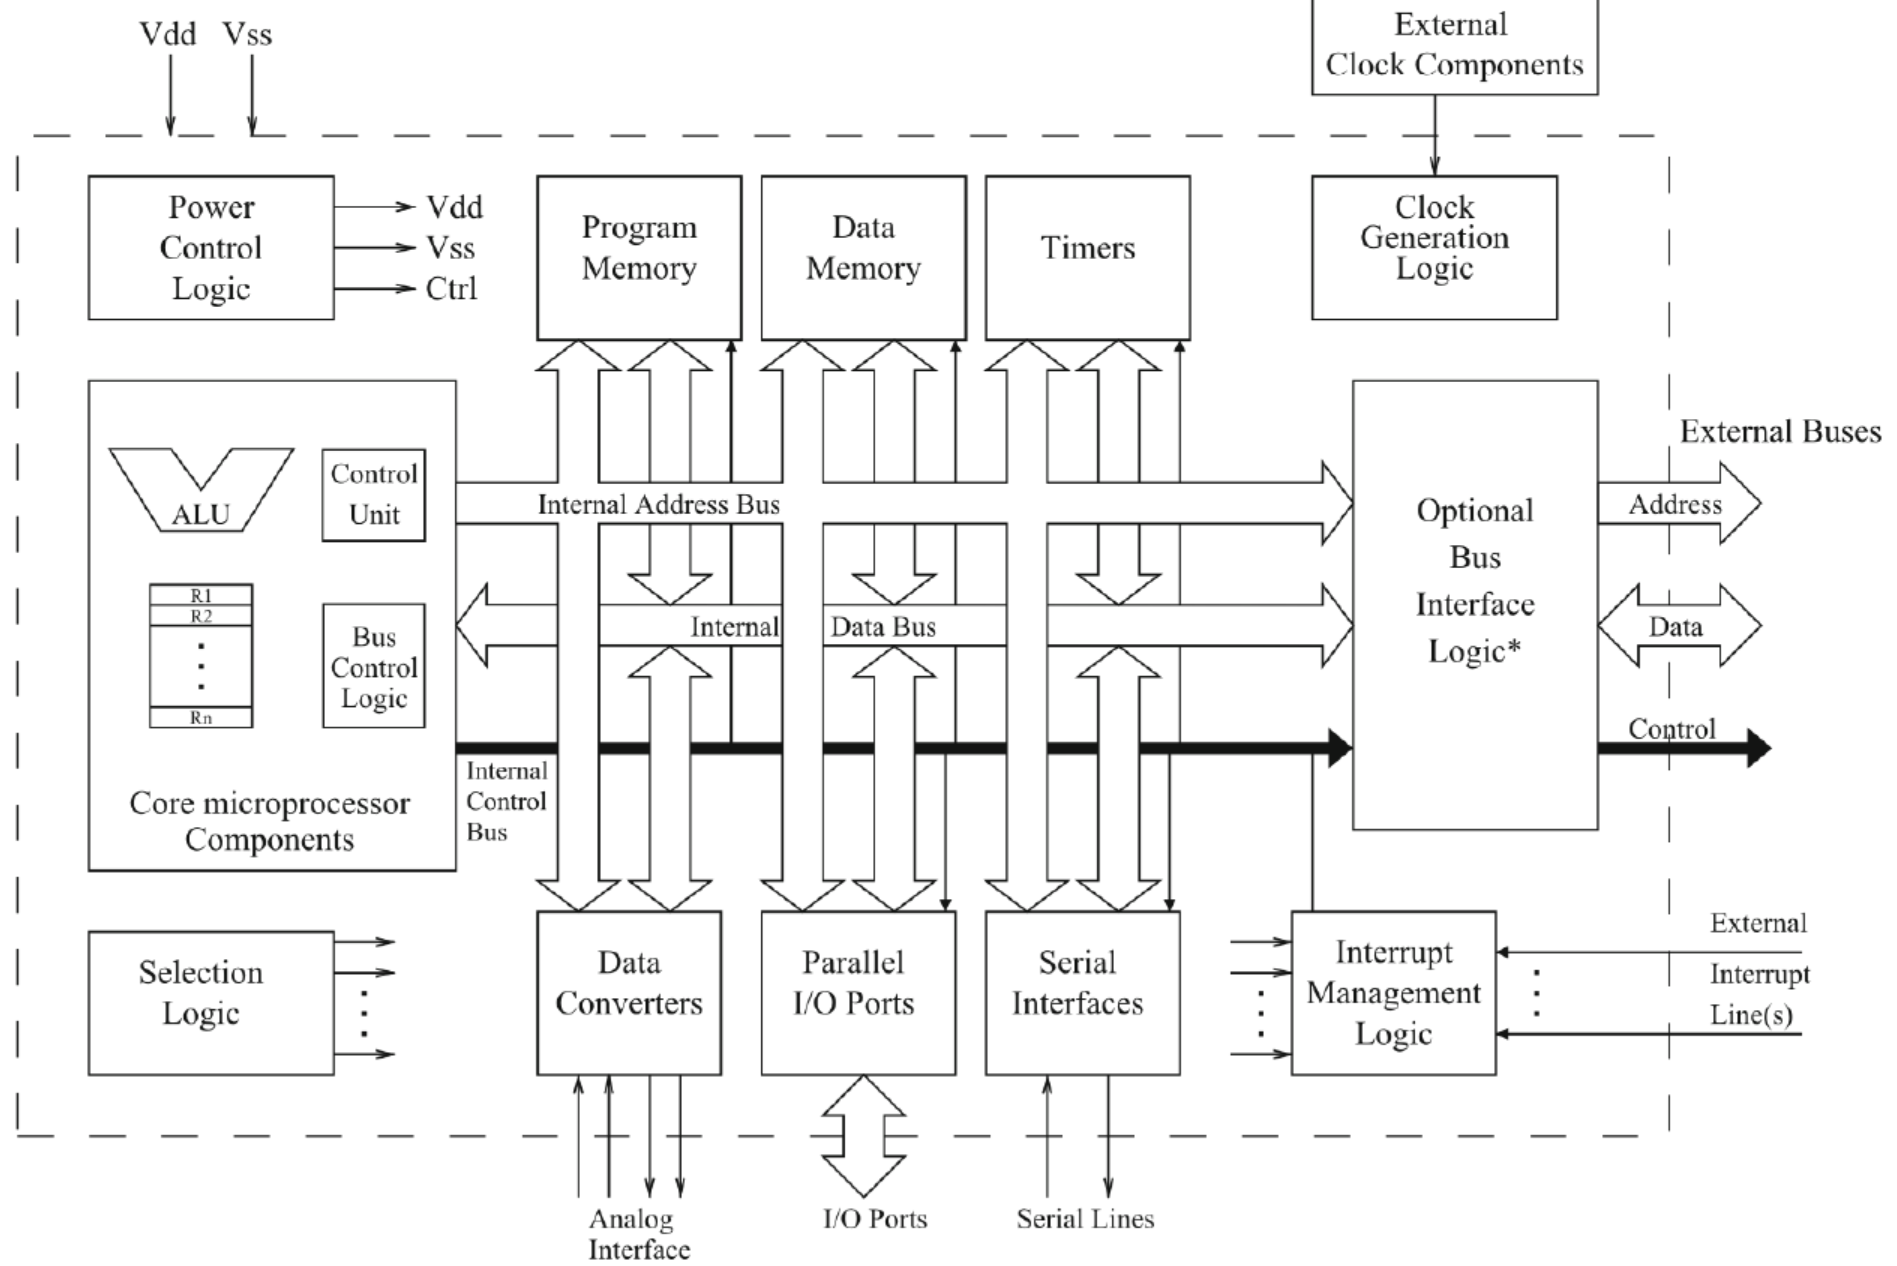
\includegraphics[width=8cm]{images/mCStructure}


\subsubsection{\acs{RISC} vs. \acs{CISC}}
\begin{multicols}{2}
	\textbf{\acs{CISC} (Complex Instruction Set Computer)}
		\begin{itemize}
			\item Variable length instructions
			\item Large instruction set
			\item Focuses in accomplishing as much as possible with each instruction
			\item Augments hardware complexity
			\item Simplifies programming
		\end{itemize} 
          \columnbreak
	\textbf{\acs{RISC} (Reduced Instruction Set Computer)}
		\begin{itemize}
			\item Fixed length insructions
			\item Short instruction set
			\item Focuses on simple instructions
			\item Simplifies the hardware structure
			\item Makes programming harder
		\end{itemize}      
\end{multicols}
\clearpage
%=====================================================


\subsection{Central Processing Unit \embsys{86}{3.3}}
\begin{multicols}{2}
\begin{minipage}{\linewidth}
	\begin{itemize}
		\item Controll Unit (\acs{CU})
		\item Arithmetic Logic Unit (\acs{ALU})
		\item Register and Flags
		\item Bus Interface Logic (\acs{BIL})
	\end{itemize}
\end{minipage}
	\subsubsection{Control Unit (\acs{CU})}   
		\begin{itemize}
			\item Governs the CPU working
			\item Name of Cycles States: Fetch, Decode, Execute
			\item Also known als Infinite Loop or while(1)
		\end{itemize}	
	\subsubsection{Arithmetic Logic Unit (\acs{ALU})}
	\begin{itemize}
		\item Performs Logic and Arithmetic Operations
		\item 'Sets' the width of Databus and Registers
	\end{itemize}	
	\subsubsection{Bus Interface Logic (\acs{BIL})}
	\begin{itemize}
		\item Coordinates interaction between internal buses and system buses
		\item Define how adress, data and control buses works
	\end{itemize}	
	\subsubsection{Registers}
	\begin{itemize}
		\item Provide temporary storage in \acs{CPU}
		\item Fastest form of storage
		\item Volatile Contents
		\item General and Special Purpose Registers
	\end{itemize}
	\subsubsection{Special Register (\acs{SR})}	
	\begin{itemize}
		\item Instruction Register (\acs{IR})
		\subitem Holds the current instruction 
		\item Programm Counter (\acs{PC})
		\subitem Holds address of next instruction fetched
		\item Stack Pointer (\acs{SP})
		\subitem Holds the address of the current top-of-stack 
		\item Status Register (\acs{SR})
		\subitem Holds the current \acs{CPU} Status (Flags)
	\end{itemize}
\vfill
\columnbreak
\begin{minipage}{\linewidth}
    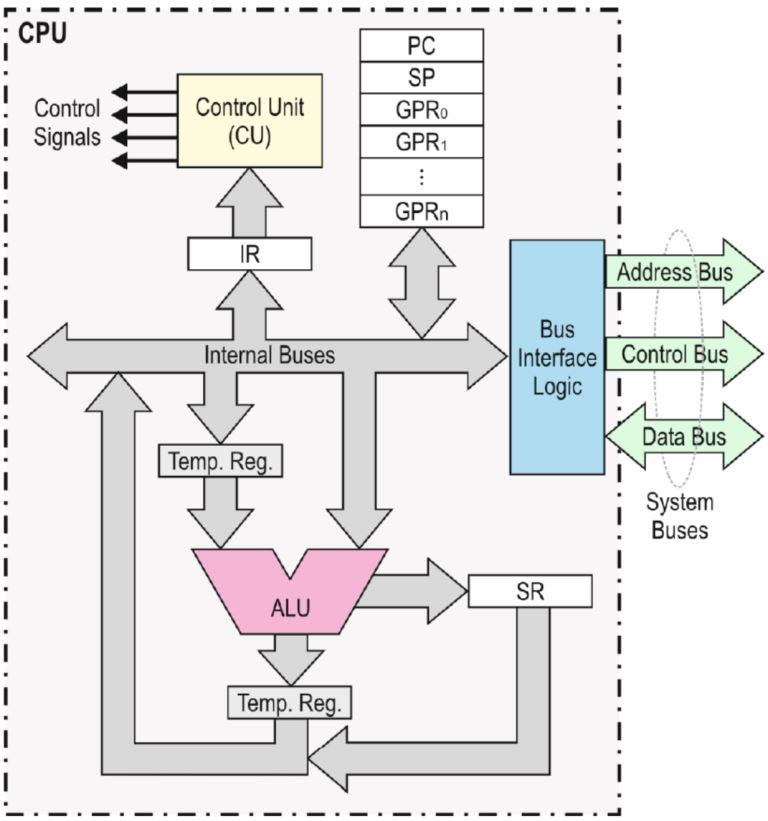
\includegraphics[width=\linewidth]{images/CPUComponents}	
\end{minipage}

	\subsubsection{Status Flags}
	\begin{itemize}
		\item Zero Flag (Z)
		\subitem Set when an \acs{ALU} Operation is zero
		\item Carry Flag (C)
		\subitem Set when an \acs{ALU} Operation produce carry
		\item Negativ or Sign Flag (N)
		\subitem Set when an \acs{ALU} Operation is negative
		\item Overflow Flag (V)
		\subitem Set when an \acs{ALU} Operation produce overflow
		\item Interrupt Flag (IF)
		\subitem Also called Global Interrupt Enable
		\subitem Is not associated to \acs{ALU} status
		\subitem Indicates whether\acs{CPU} accept interrupts
	\end{itemize}

	\subsubsection{General Purpose Regiser (\acs{GPR})}
    \begin{itemize}
        \item Not tied to specific functions
        \item Can hold data, variables, or addresses
        \item Number of registers depend on \acs{CPU} architecture			
    \end{itemize}

\end{multicols}
\subsection{System Buses \embsys{96}{3.4}}
\vspace{-0.3cm}
	\begin{multicols}{2}
	\begin{itemize}
		\item Data Bus
		\subitem carrying data \& instructions for read \&write
		\subitem bidirectional \acs{CPU} $\leftrightarrow$ \acs{I/O} or memory
		\item Adress bus
		\subitem Indicate Adress to be accessed
		\subitem number of memory which is adressable: 
		\subitem 16 Bit Bus $\rightarrow 2^{16}=64kB$ Memory
		\subitem \textbf{Data Adress:}
		\subitem The address of the first byte of a data item
		\subitem \textbf{Physical Adress:} 
		\subitem The address of each memory location
		\item Control bus
		\subitem regulate activity on buses		
	\end{itemize}
	\end{multicols}
\clearpage
%====================================================

\subsection{Memory Organization \embsys{98}{3.5}}
\begin{minipage}{9cm}
		\begin{itemize}
			\item The memory is organized as an array of cells
			\item Each memory location is identified by an adress
			\item The contents of a memory cell is a word
		\end{itemize}
    
\subsubsection{Bus Architecture}
    \begin{itemize}
        \item Von Neumann
        \subitem A single bus for Instructions and Data
        \item Harvard
        \subitem Separate Bus for Instructions and Data
    \end{itemize}
\end{minipage}
\begin{minipage}{8cm}
    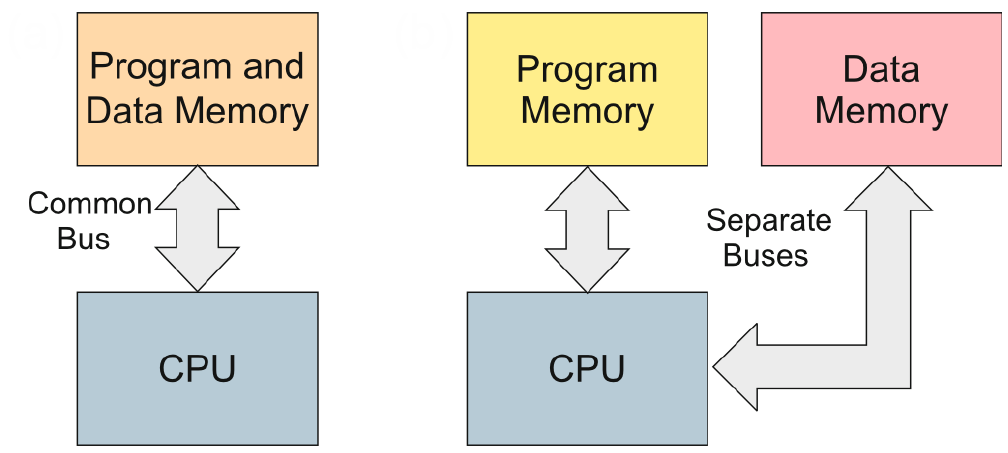
\includegraphics[width=\linewidth]{images/bus}
\end{minipage}

\begin{multicols}{2}
\subsubsection{Memory Types}
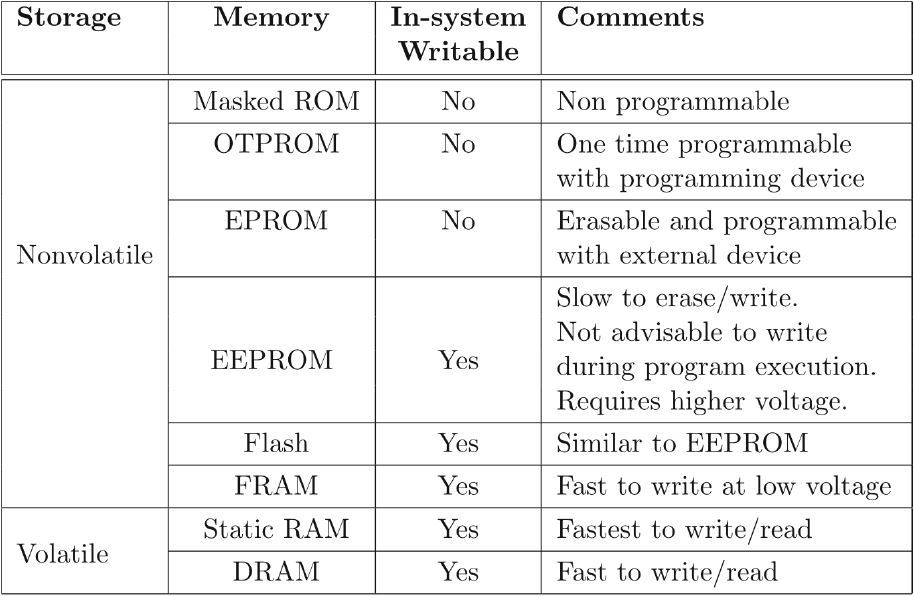
\includegraphics[width=9cm]{images/memorytypes}

\subsubsection{Endianness}
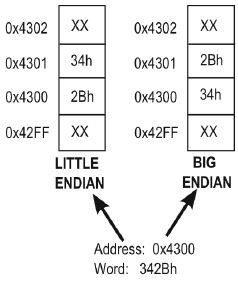
\includegraphics[width=4.5cm]{images/be_le}
\end{multicols}

\subsection{I/O Subsystem \embsys{109}{3.6}}
Convers all the components other than the \acs{CPU} \& memory connected to the system buses
\begin{itemize}
	\item Timers and Watchdog timers
	\item Communication interfaces
	\item Analog to Digital Converter (\acs{ADC})
	\item Digital to Analog Converter (\acs{DAC})
	\item Development peripherals
\end{itemize}
\begin{multicols}{2}
	\begin{minipage}{\linewidth}
		\subsubsection{Memory mapped \acs{I/O}}
		Address space inside the memory space, uses same instructions used to access memory
	\end{minipage}	
	\begin{minipage}{\linewidth}
		\subsubsection{\acs{I/O} mapped \acs{I/O}}
		Separate address space, instrutions, and signals for \acs{I/O} (rarley used in modern processors)
	\end{minipage}
\end{multicols}
\begin{minipage}{0.6\linewidth}
	\subsubsection{\acs{I/O} Interface}
	\raggedright
	Include lines to connect to the system buses, \acs{I/O} device connection lines and a set of internal registers
	\begin{tabular}{ll}
		\textbf{Control}  & to configure the operation of the device and interface  \\  
		\textbf{Status}   & to allow inquires about the device and interface status  \\ 
		\textbf{Data}     & for exchanging data with the device \\ 
	\end{tabular} 
\end{minipage}
\begin{minipage}{0.4\linewidth}
	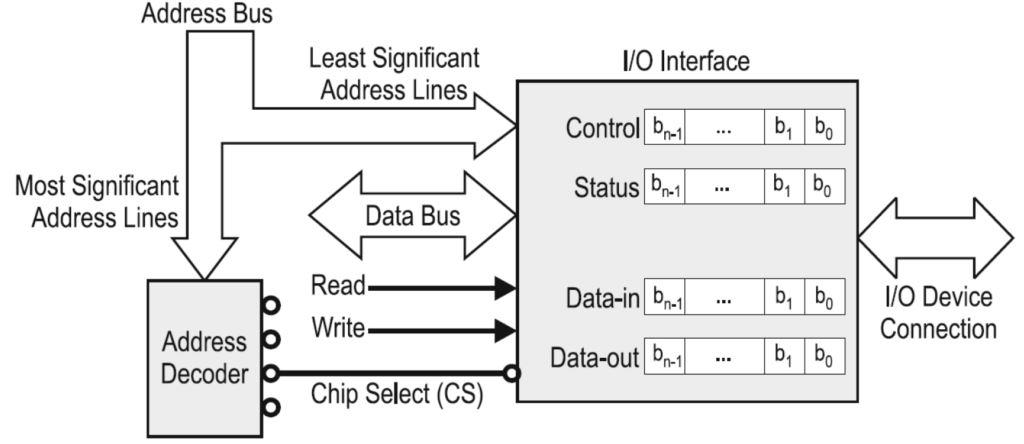
\includegraphics[width=\linewidth]{images/IOAnatomy} 
\end{minipage}
\clearpage
\pagebreak
